\section{File Systems}

\paragraph{File Systems --- motivation}
\begin{itemize}
  \item \textbf{goal}: enable storing of large data amounts \\*
    $ - $ store data/program consistently + persistently \\*
    $ - $ easily look up previously stored data/program
  \item \textbf{file types}: \\*
    $ - $ \emph{data} (numeric, character, binary) \\*
    $ - $ \emph{program}
\end{itemize}

\paragraph{File Systems --- overview}
\begin{itemize}
  \item OS may support multiple file systems
  \item \textbf{namespace}: all file systems typically bound into single namespace (often hierarchical, rooted tree)
\end{itemize}

\paragraph{Files -- abstract operations}
\begin{itemize}
  \item \textbf{file}: abstract data type/object, offering \\*
    $ - $ \code{create}, \code{write}, \code{read}, \\*
    $ - $ \code{reposition} (within file), \\*
    $ - $ \code{delete}, \code{truncate}, \\*
    $ - $ \code{open(}$ F_i $\code{)} (search directory structure on disk for entry $ F_i $, move meta data to memory),  \\*
    $ - $ \code{close(}$ F_i $\code{)} (move cached meta data of entry $ F_i $ in memory to directory structure on disk)
\end{itemize}
\begin{figure}[h]\centering\label{FileSystemInteraction}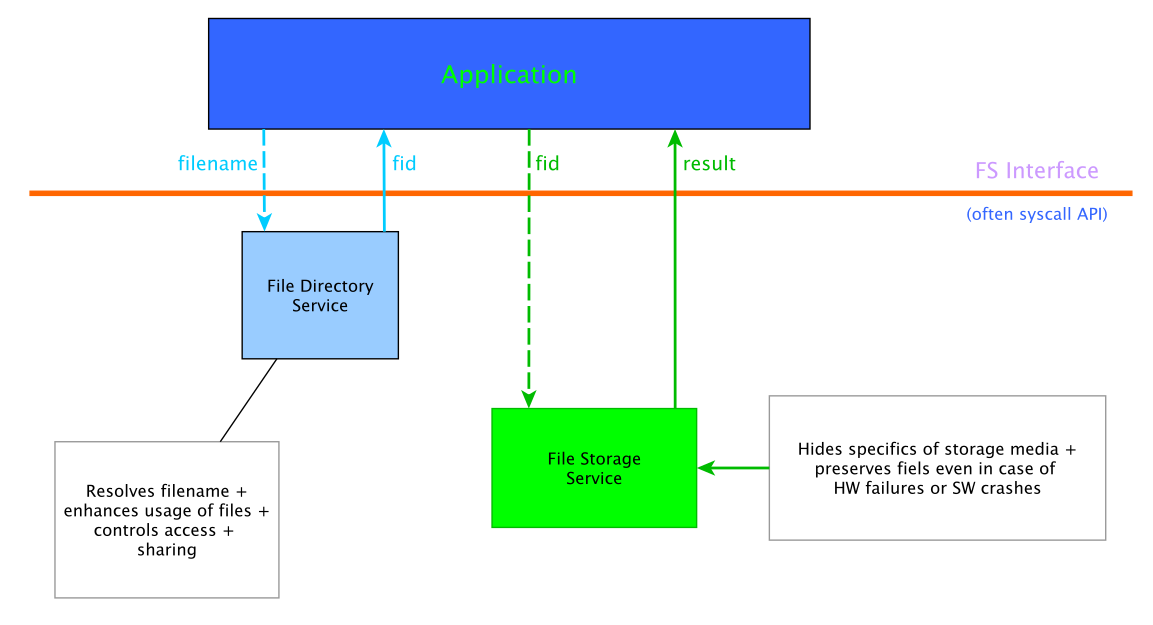
\includegraphics[width=0.4\textwidth]{FileSystemInteraction}\end{figure}

\paragraph{File Management --- goals}
\begin{itemize}
  \item provide convenient file naming scheme
  \item provide uniform I/O support for variety of storage device types
  \item provide standardized set of I/O interface functions
  \item minimize/eliminate loss/corruption of data
  \item provide I/O support + access control for multiple users
  \item enhance system administration (e.g., backup)
  \item provide acceptable performance
\end{itemize}

\paragraph{File Management --- open files}
\begin{itemize}
  \item several meta data is needed to manage open files
  \item \textbf{file pointer}: pointer to last read/write location, per process that has file opened
  \item \textbf{access rights}: per-process access mode information
  \item \textbf{file-open count}: counter of number of times a file is opened (to allow removal of data from open-file table when last process closes)
  \item \textbf{disk location}: cache of data access information
\end{itemize}

\paragraph{File Access}
\begin{itemize}
  \item \textbf{strictly sequential} (early systems): \\*
    $ - $ read all bytes/records from beginning \\*
    $ - $ cannot jump round, could only rewind \\*
    $ - $ sufficient as long as storage was a tape
  \item \textbf{random access} (current systems): \\*
    $ - $ bytes/records read in any order \\*
    $ - $ essential for database systems
\end{itemize}

\paragraph{Directories --- goals}
\begin{itemize}
  \item \textbf{naming}: convenient to users \\*
    $ - $ two users can have same name for different files \\*
    $ - $ same file can have several different names
  \item \textbf{grouping}: logical grouping of files by properties
  \item \textbf{efficiency}: fast operations
\end{itemize}

\paragraph{Files --- sharing}
\begin{itemize}
  \item \textbf{issues}: \\*
    $ - $ efficiently access to same file? \\*
    $ - $ how to determine access rights? \\*
    $ - $ management of concurrent accesses?
  \item \textbf{access rights}: \\*
    $ - $ \emph{none}: existence unknown to user, user cannot read directory containing file \\*
    $ - $ \emph{knowledge}: user can only determine existence and file ownership \\*
    $ - $ \emph{execution}: user can load + execute program, but can not copy it \\*
    $ - $ \emph{reading}: user can read file (includes copying + execution) \\*
    $ - $ \emph{appending}: user can only add data to file, but cannot modify/delete data in file \\*
    $ - $ \emph{updating}: user can modify + delete + add to file (includes creating + removing all data) \\*
    $ - $ \emph{change protection}: user can change access rights granted to other users \\*
    $ - $ \emph{deletion}: user can delete file \\*
    $ - $ \emph{owner}: all previous rights + rights granting
  \item \textbf{concurrent access}: \\*
    $ - $ \emph{application locking}: application can lock entire file or individual records for updating \\*
    $ - $ \emph{exclusive vs. shared}: writer lock vs. multiple readers allowed \\*
    $ - $ \emph{mandatory vs. advisory}: access denied depending on locks vs. process can decide what to do
\end{itemize}